% Section content template for individual Educative lessons
% This file contains the actual content for a specific section
% Generated from Educative API section content

% Section: Class Diagram for the Online Blackjack Game
% Section ID: 4902989846544384
% Section Slug: class-diagram-for-the-online-blackjack-game
% Generated: 2025-12-12T12:36:51.034375

In this lesson, we'll create the class diagram for the Blackjack game. We will first define the core classes, then identify their relationships to fully model the game's structure according to our requirements.

\subsection{Components of Blackjack}\label{MdHRuuDazoecrq0w5P6EH}
\\
In this section, we'll define the classes for the Blackjack game. As mentioned earlier, we are following the bottom-up approach to designing a class diagram for the Blackjack game.

\subsubsection{Card}\label{ipIO4X3pjxbTgOsHHwWrx}
\\
The \texttt{Card} class encapsulates the properties of a single playing card used in Blackjack. Each
\texttt{Card} object is defined by its suit (hearts, spades, clubs, or diamonds) and face value (ranging from Ace to King). The class includes methods to determine the card's Blackjack point value (with special handling for face cards and Aces) and to provide a human-readable string representation of the card.

\begin{figure}[htbp]
 \centering
 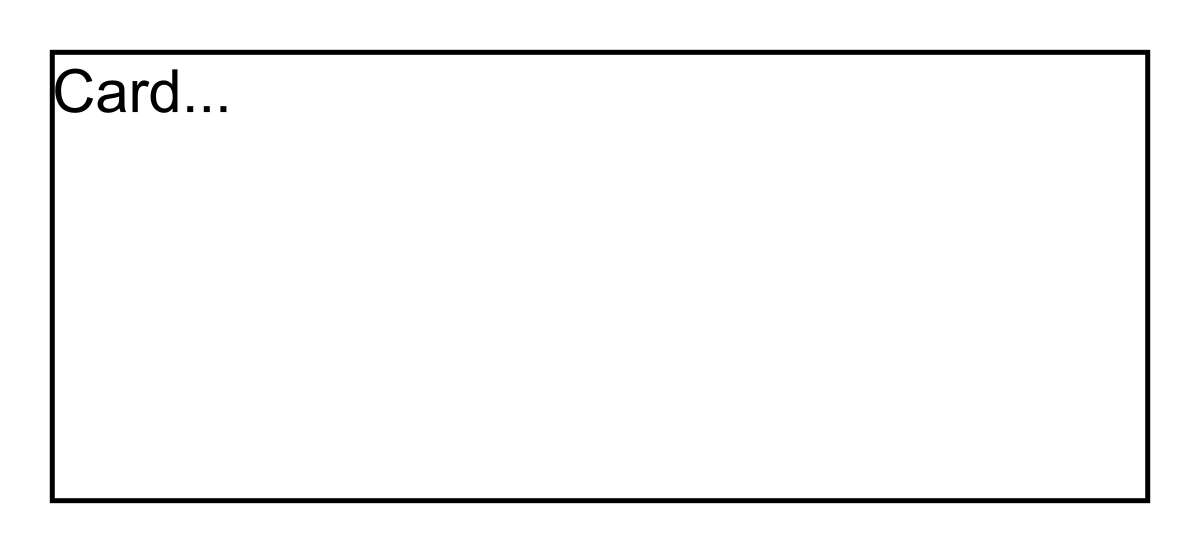
\includegraphics[width=0.5\textwidth]{Images/chapter_12/section_4902989846544384/5545265338384384.png}
 \caption{The class diagram of the Card class}
\end{figure}

\textbf{R2:} Each deck consists of 52 cards in four suits (Hearts, Diamonds, Clubs, Spades), each containing 13 ranks: Ace, 2--10, Jack, Queen, and King.
\\
\textbf{R3:} Every card has a specific point value:

\begin{itemize}
\tightlist
\item
\textbf{Ace:} values equal 1 or 11
\item
\textbf{Number cards from 2 to 10:} values equal to their numbers
\item
\textbf{Face cards:} value equals 10 for each
\end{itemize}

\subsubsection{Deck}\label{QpxIqWSVswoqdlNZHDjVH}
\\
The \texttt{Deck} class represents a standard 52-card playing deck, consisting of all possible suit and face value combinations. Upon instantiation, a deck automatically populates with \texttt{Card} objects for each unique combination. Deck provides access to its list of cards, enabling shuffling, dealing, and integration into larger components like the \texttt{Shoe} class.

\begin{figure}[htbp]
 \centering
 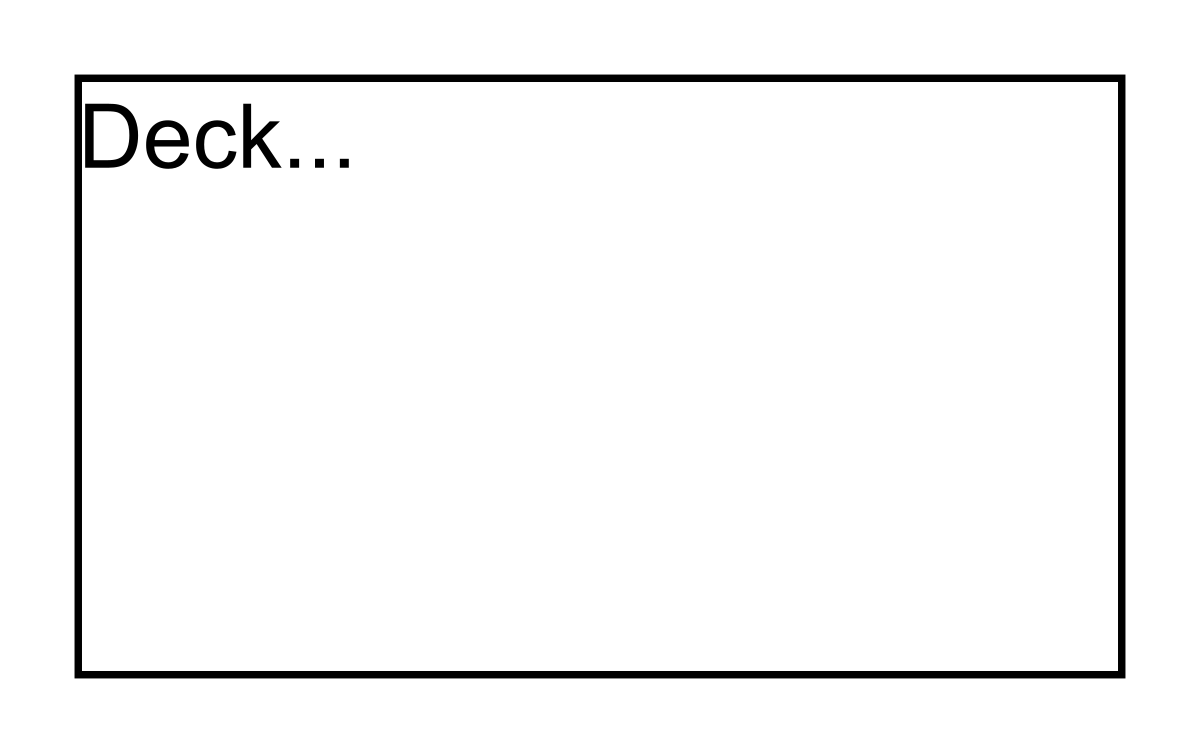
\includegraphics[width=0.5\textwidth]{Images/chapter_12/section_4902989846544384/5284296112603136.png}
 \caption{The class diagram of the Deck class}
\end{figure}

\textbf{R2:} Each deck consists of 52 cards in four suits (Hearts, Diamonds, Clubs, Spades), each containing 13 ranks: Ace, 2--10, Jack, Queen, and King.

\subsubsection{Shoe}\label{pvOhIO4D3aHzzk4Pqr4_p}
\\
The \texttt{Shoe} class models the casino device that holds multiple shuffled decks of cards. It is the source for all card dealing during the game, ensuring a large enough card supply for extended play and fair distribution. The
\texttt{Shoe} is responsible for initializing itself with the required number of decks, shuffling all the cards together, and providing cards one at a time for dealing to players and the dealer.

\begin{figure}[htbp]
 \centering
 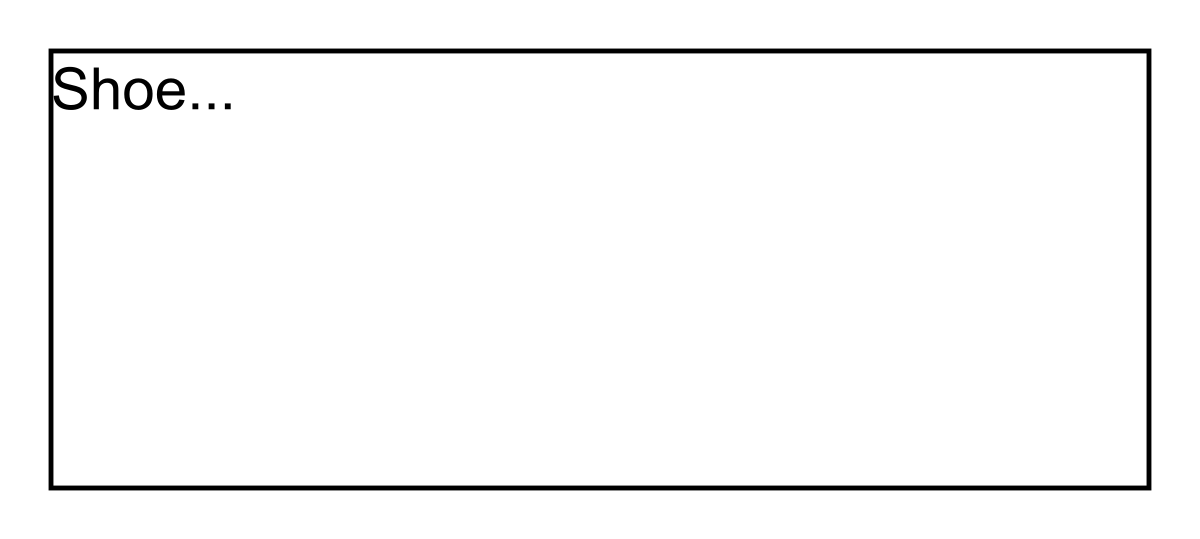
\includegraphics[width=0.5\textwidth]{Images/chapter_12/section_4902989846544384/4644861691953152.png}
 \caption{The class diagram of the Shoe class}
\end{figure}

\textbf{R1:} The system must support a shoe containing one or more standard decks of cards.

\subsubsection{Hand}\label{HU1isNs4rzhKJ34H8hJlV}
\\
The \texttt{Hand} class represents the collection of cards a player or dealer currently holds in a single round of Blackjack. It provides operations for adding new cards and computing the hand's total point value, with intelligent handling of the Ace's dual value (1 or 11) to optimize for the best score without busting.

\begin{figure}[htbp]
 \centering
 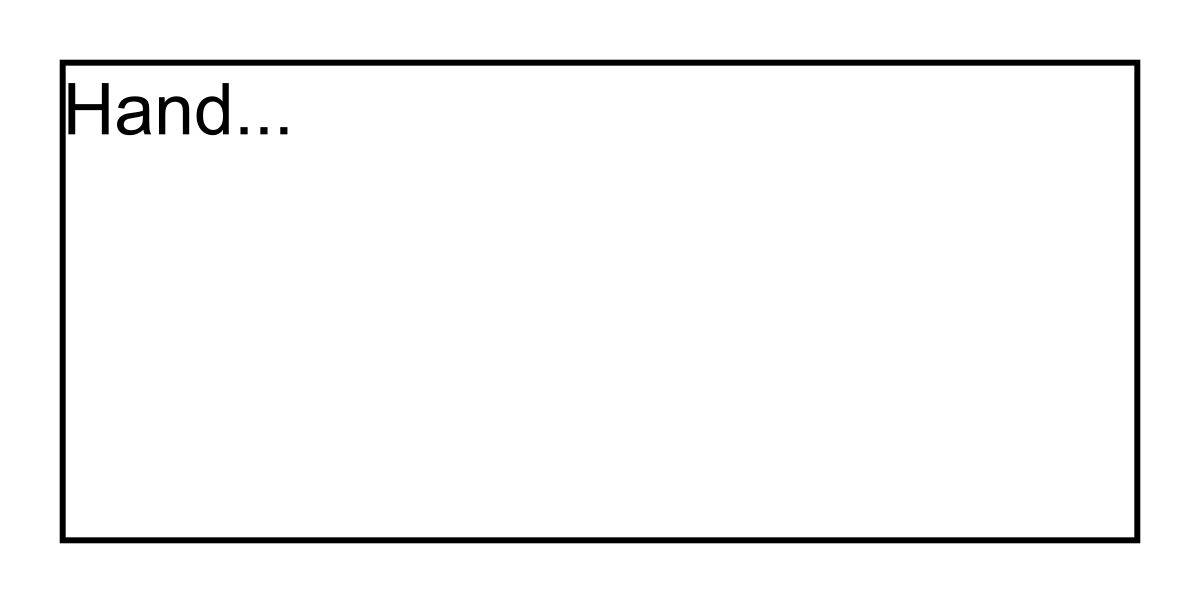
\includegraphics[width=0.5\textwidth]{Images/chapter_12/section_4902989846544384/4615240283979776.png}
 \caption{The class diagram of the Hand class}
\end{figure}

\textbf{R3:} Every card has a specific point value:

\begin{itemize}
\tightlist
\item
\textbf{Ace:} values equal 1 or 11
\item
\textbf{Number cards from 2 to 10:} values equal to their numbers
\item
\textbf{Face cards:} value equals 10 for each
\end{itemize}
\\
\textbf{R8:} Players may hit (draw an additional card) if their hand total is less than 21 points.
\\
\textbf{R9:} According to standard Blackjack rules, the dealer must hit if their hand value exceeds 17 points.
\\
\textbf{R10:} If a player's or dealer's hand exceeds 21 points, they bust and immediately lose that round.

\subsubsection{Player, BlackjackPlayer, and Dealer}\label{Jwiq3PRzNByxP8Hyrszb4}
\\
The \texttt{Player} class is an abstract base class that encapsulates all the common attributes and behaviors shared by participants in the Blackjack game. Each player maintains identifying information, login credentials, account status, a running cash balance, and a reference to their personal details through the \texttt{Person} object. The
\texttt{Player} class is also associated with a \texttt{Hand}, representing the current set of cards held by that participant in any round.

\begin{itemize}
\item
\protect\phantomsection\label{sjk-AjK45q_BMduuOFz6S}
\textbf{\texttt{BlackjackPlayer}:} This class represents a human participant who joins the Blackjack game to place wagers and compete against the dealer. Extending from the \texttt{Player} base class, \texttt{BlackjackPlayer} adds capabilities specific to casino play, such as tracking the amount of the current bet amount, updating the total cash balance after each win or loss, and managing the logic for payouts according to Blackjack's rules.
\item
\protect\phantomsection\label{vutRSL1Gzd35eGDT24s7r}
\textbf{\texttt{Dealer}:} This class models the role of the house representative in a Blackjack game. Inheriting from the \texttt{Player} base class, \texttt{Dealer} manages the game's flow according to standard casino procedures. This includes dealing the initial cards to all participants, maintaining the dealer's hand, and executing all dealer-specific rules---such as drawing cards until reaching a minimum hand value (usually 17).
\end{itemize}

\begin{figure}[htbp]
 \centering
 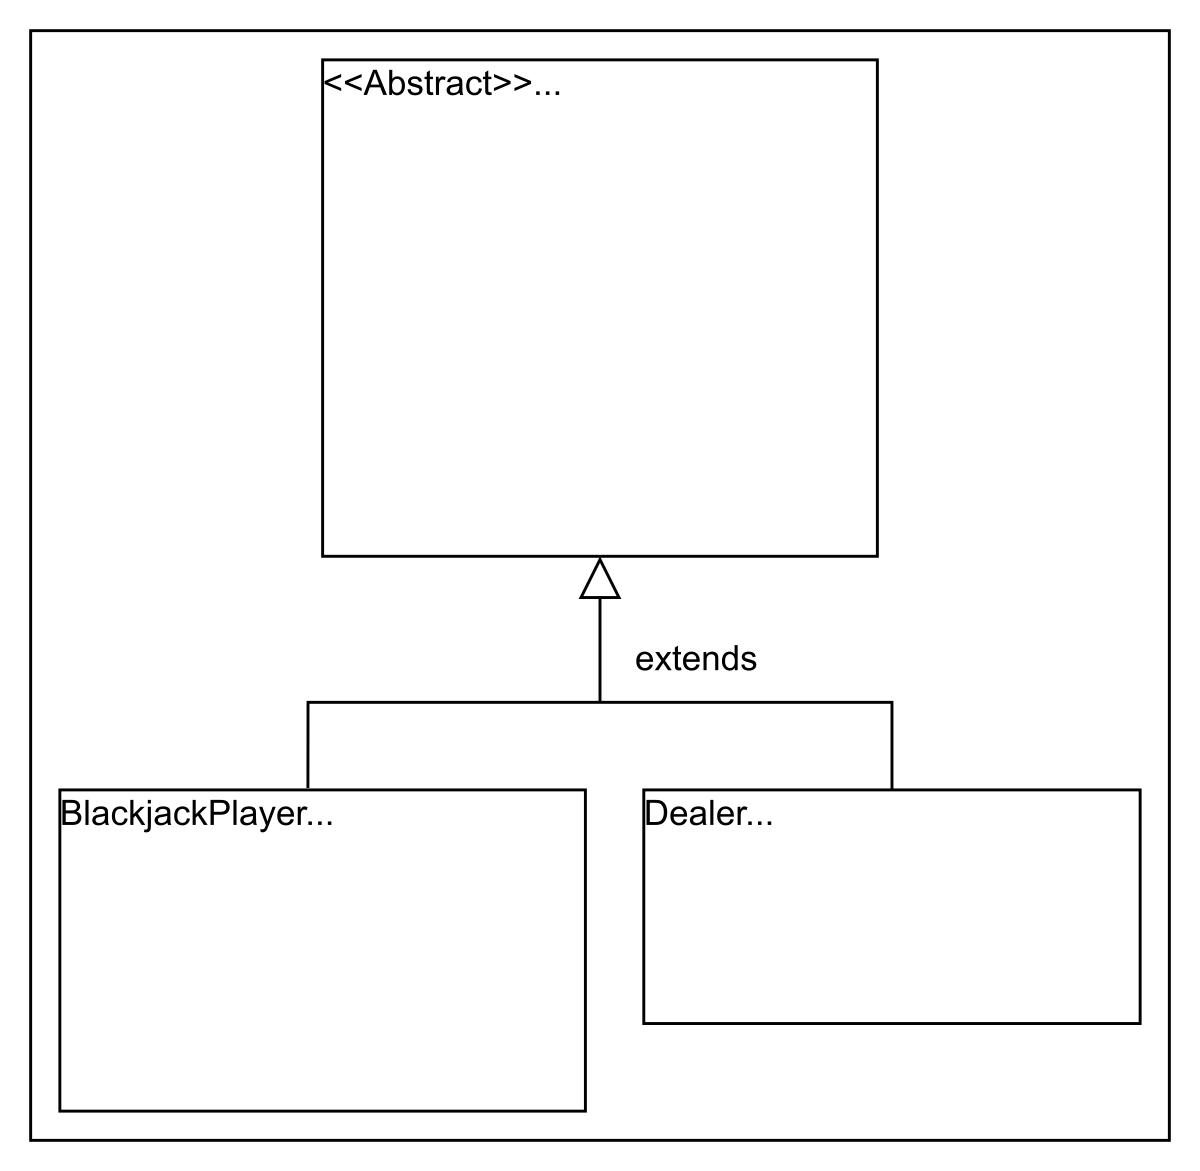
\includegraphics[width=0.5\textwidth]{Images/chapter_12/section_4902989846544384/6482047307481088.png}
 \caption{The class diagram of Player and its derived classes}
\end{figure}

\textbf{R4:} Two types of users can play the Blackjack game, i.e., the dealer and the player.

\subsubsection{BlackjackController}\label{XMKS3vSe2KaLfgHm7vxLW}
\\
The \texttt{BlackjackController} class acts as the mediator between the player's actions and the core game logic. It is responsible for validating player decisions (such as whether a requested action is legal at a given point in the game) and processing those actions according to the rules.

\begin{figure}[htbp]
 \centering
 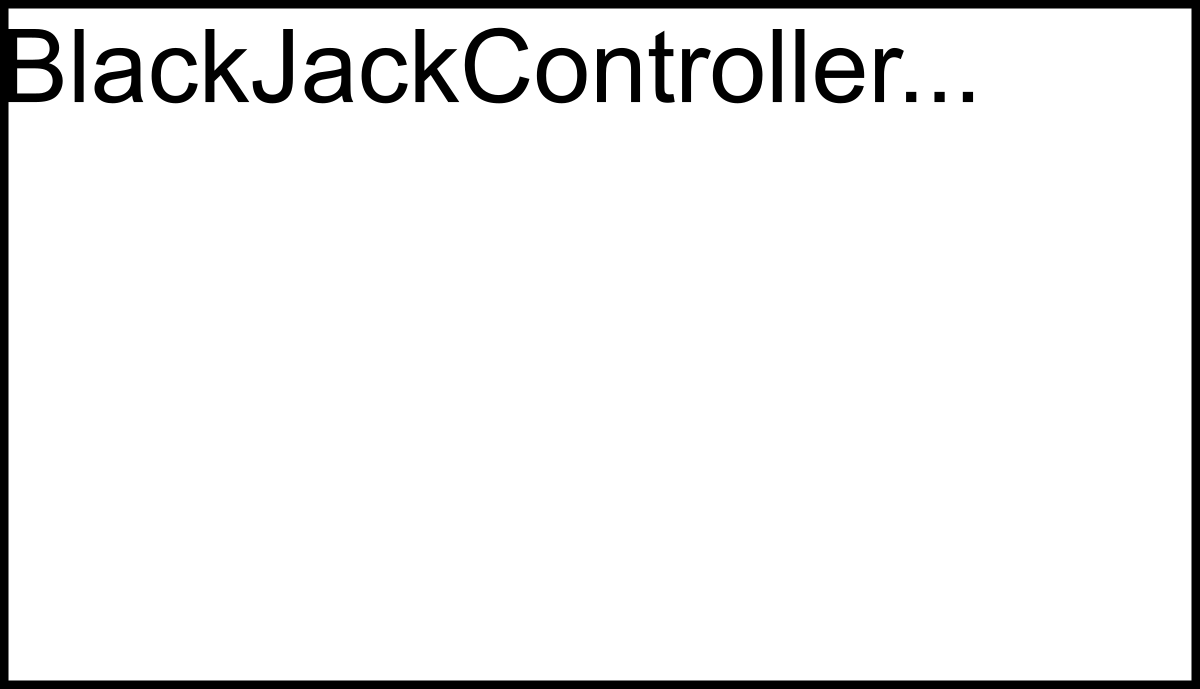
\includegraphics[width=0.5\textwidth]{Images/chapter_12/section_4902989846544384/6084485483593728.png}
 \caption{The class diagram of the BlackjackController class}
\end{figure}

\subsubsection{BlackjackGameView}\label{MmpALo4VW7Ea5vwfxVPLW}
\\
The \texttt{BlackjackGameView} class handles all aspects of displaying the game's state to the players. It receives updates from the game logic and presents key information such as the current hands, dealer's exposed cards, round results, and payouts. This class ensures that players are always informed of their status and the outcome of each game event in a clear and timely manner.

\begin{figure}[htbp]
 \centering
 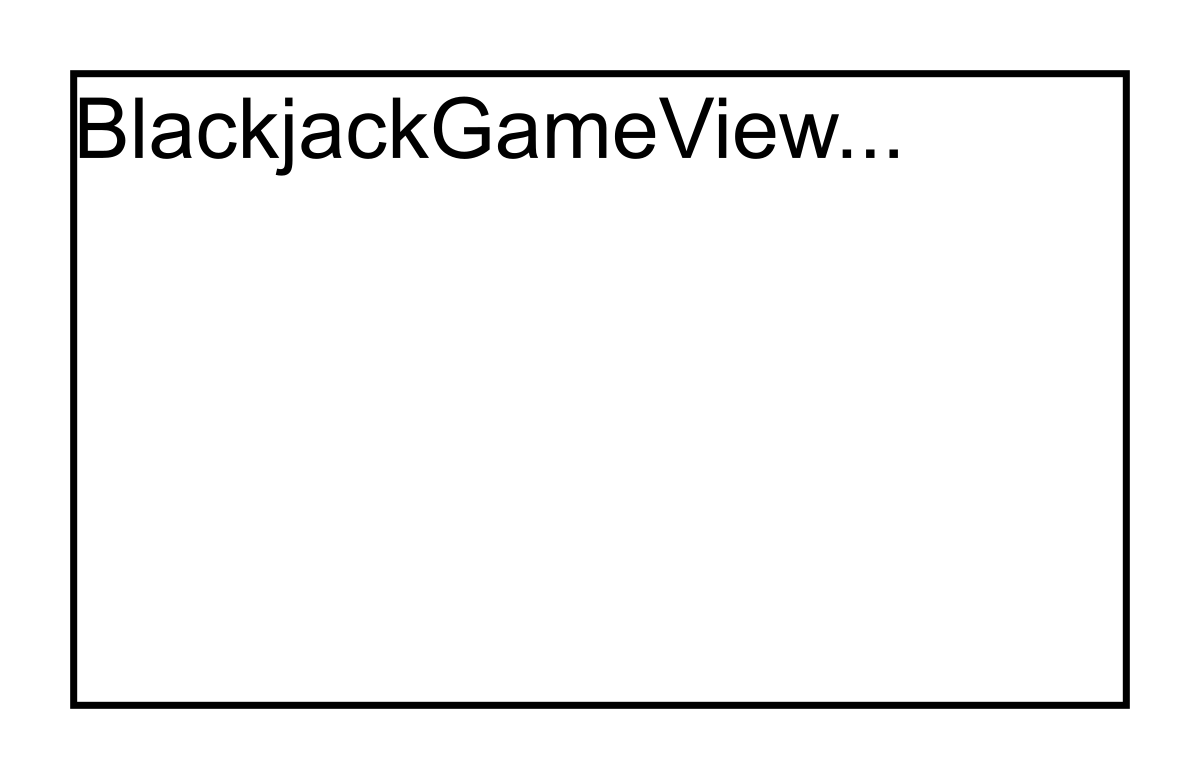
\includegraphics[width=0.5\textwidth]{Images/chapter_12/section_4902989846544384/5863469097025536.png}
 \caption{The class diagram of the BlackjackGameView class}
\end{figure}

\subsubsection{BlackjackGame}\label{YNTuAT6neTwPHorAY8P_S}
\\
The \texttt{BlackjackGame} class is the central orchestrator for the entire game session. It manages the main sequence of play, ensuring the correct flow of each game round. This class is responsible for initializing the game with the necessary players, dealer, and shuffled shoe of cards. It accepts wagers from players, distributes cards from the Shoe to players' and the dealer's hands, and updates the game's status throughout the round.
\\
During gameplay, \texttt{BlackjackGame} processes all player decisions---such as hit or stand---by invoking the necessary logic and enforcing Blackjack rules. It manages the collection of lost wagers, calculates and pays out winnings, and ensures that the dealer's actions (such as revealing the hole card and drawing to 17) follow standard casino rules. The class also interacts with the game view component to keep players informed about the current state of play and the results of each round. This makes \texttt{BlackjackGame} the backbone, seamlessly integrating all other components and driving the game's logic forward.

\begin{figure}[htbp]
 \centering
 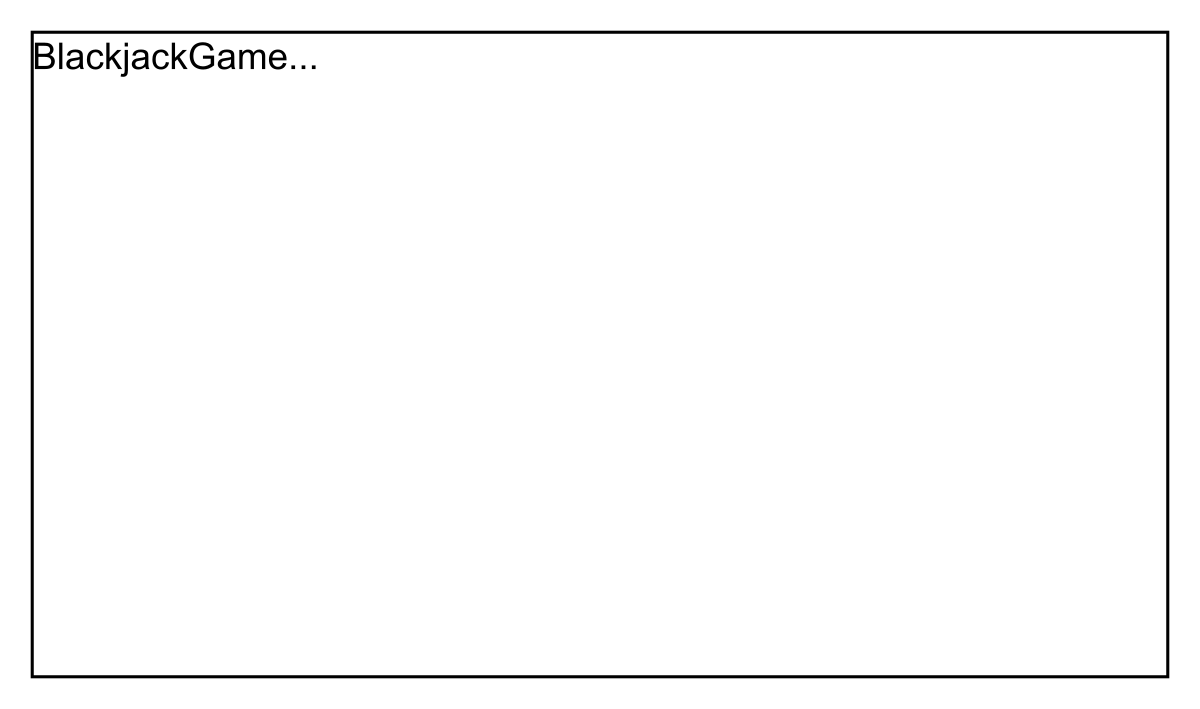
\includegraphics[width=0.5\textwidth]{Images/chapter_12/section_4902989846544384/5701111380836352.png}
 \caption{The class diagram of the BlackjackGame class}
\end{figure}

All requirements from \textbf{R5} to \textbf{R15}.

\subsubsection{Enumerations and custom data types}\label{MWdMsKN-a5RBDxDdmvW0X}
\\
The following provides an overview of the enumerations and custom data types used in this problem:

\begin{itemize}
\item
\protect\phantomsection\label{W39ZxFQpRZlqHaL232Jy6}
\texttt{Suit:}~The \texttt{Suit} enumeration defines the four standard suits found in a deck of cards---Hearts, Spades, Clubs, and Diamonds. It provides a type-safe way to assign and compare suits across the system.
\item
\protect\phantomsection\label{UzkXmOpptZydZfQyzbobp}
\texttt{AccountStatus:}~The \texttt{AccountStatus} enumeration captures the possible states of a player or dealer account, such as active, closed, canceled, blocklisted, or none. This supports account management logic, restricting access or play when required.
\end{itemize}

\begin{figure}[htbp]
 \centering
 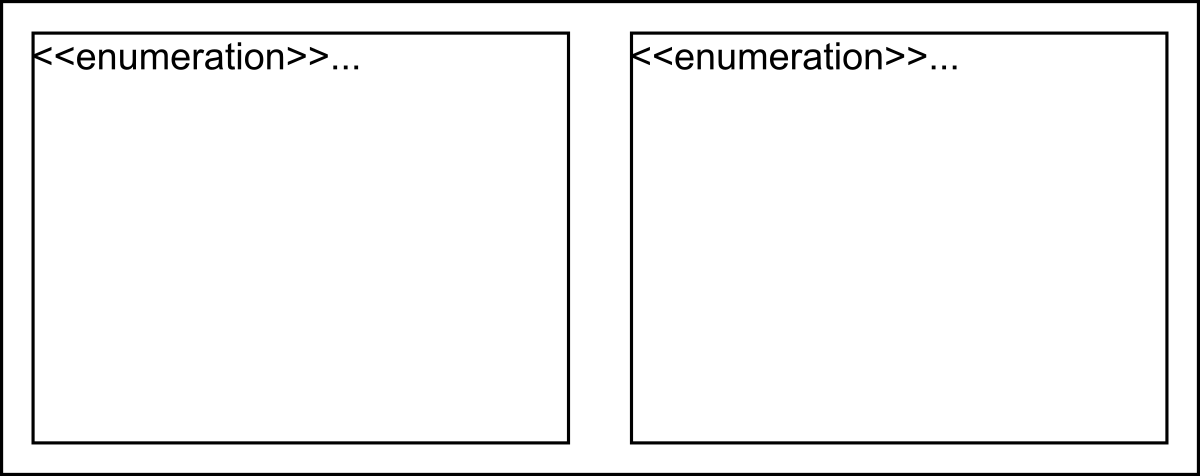
\includegraphics[width=0.5\textwidth]{Images/chapter_12/section_4902989846544384/5655942810304512.png}
 \caption{Enums in the Blackjack game}
\end{figure}

\begin{itemize}
\item
\protect\phantomsection\label{cWJm3LHTbrdvsHnVXhzs9}
\texttt{Person:}~The \texttt{Person} class stores personal identification and contact details for each participant (player or dealer) in the system. It holds fields such as name, address, city, state, zip code, and country. Person objects are associated with player accounts, supporting account management, record-keeping, and potential regulatory compliance.
\end{itemize}

\begin{figure}[htbp]
 \centering
 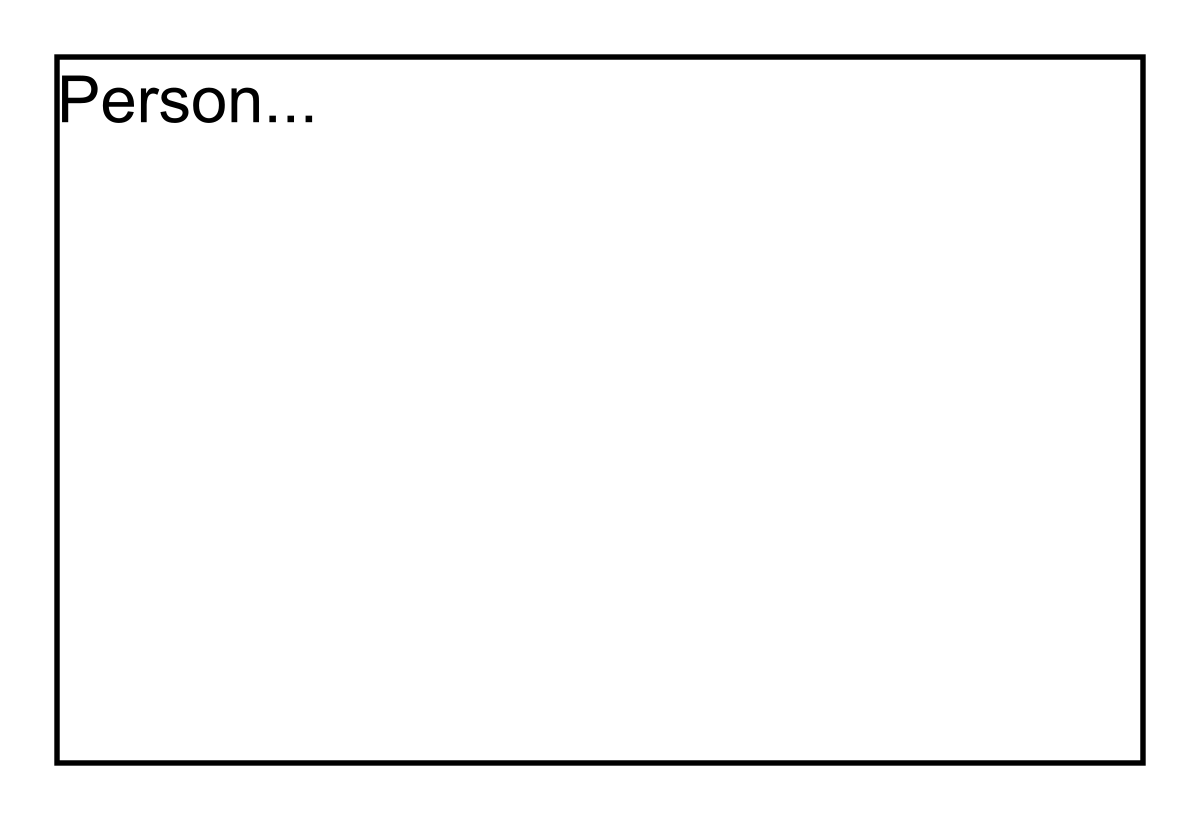
\includegraphics[width=0.5\textwidth]{Images/chapter_12/section_4902989846544384/5324631090003968.png}
 \caption{The class diagram of the Person class}
\end{figure}

\subsection{Relationship between the classes}\label{lTqA4q4Rq1gELYLeamRjz-3}
\\
Now, we'll discuss the relationships between the classes we have defined above in our Blackjack game.

\subsubsection{Association}\label{37dTwo-y_6LXSKqh8hM8g}
\\
The class diagram has the following association relationships:

\begin{itemize}
\item
\protect\phantomsection\label{J-u-yI9JkgLkXziWE9TzS}
\texttt{BlackjackGame} has an association with \texttt{BlackjackController} and \texttt{BlackjackGameView}:

\begin{itemize}
\item
Calls methods to control play and to display the game state and results.
\item
These are collaborating components, with the game logic relying on the controller to validate moves and the view to display outcomes.
\end{itemize}
\end{itemize}

\begin{figure}[htbp]
 \centering
 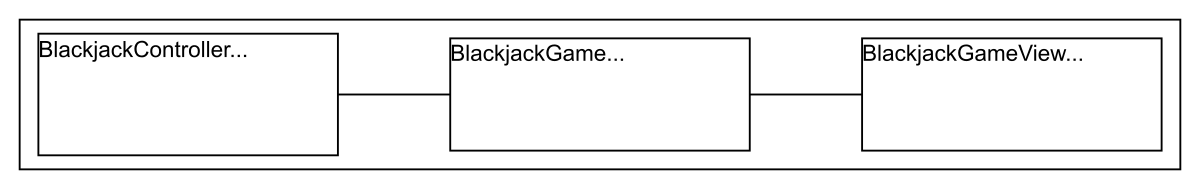
\includegraphics[width=0.5\textwidth]{Images/chapter_12/section_4902989846544384/5002821135892480.png}
 \caption{The association relationship between classes}
\end{figure}

\subsubsection{Aggregation}\label{MlZT9fkgjWl1Oxs2sk5c4}
\\
The class diagram has the following aggregation relationships.

\begin{itemize}
\item
\protect\phantomsection\label{BNQR5QGg2A9bjCGXLWE-N}
\texttt{Shoe} is an aggregation of cards:

\begin{itemize}
\item
The shoe holds all cards for the current session, sourced from one or more decks. Cards exist independently of the shoe (they can be part of other components, like the deck).
\end{itemize}
\item
\protect\phantomsection\label{BZ_fbB3z5eNyAOeguLFS_}
\texttt{Deck} is anaggregation ofcards:

\begin{itemize}
\item
A deck collects 52 cards together. The relationship is weaker than composition; cards can exist outside a deck (for example, when dealt).
\end{itemize}
\item
\protect\phantomsection\label{e92pUfjhqsc_qQiQzaMUQ}
\texttt{Hand} is anaggregation ofcards:

\begin{itemize}
\item
A hand groups together the cards a player or dealer holds during a round.
\end{itemize}
\end{itemize}

\begin{figure}[htbp]
 \centering
 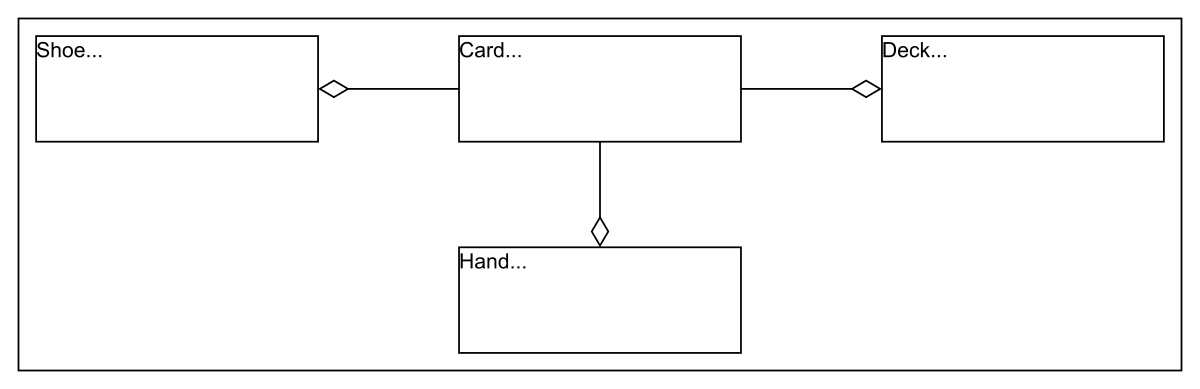
\includegraphics[width=0.5\textwidth]{Images/chapter_12/section_4902989846544384/6652609828880384.png}
 \caption{The aggregation relationship between classes}
\end{figure}

\subsubsection{Composition}\label{j9LKUkNT_QebF_q9mWfLi}
\\
The class diagram has the following composition relationships.

\begin{itemize}
\item
\protect\phantomsection\label{dyVjwp_QcCnZ_YA6YCDYI}
\texttt{BlackjackGame} is composed of:

\begin{itemize}
\item
\texttt{BlackjackPlayer}
\item
\texttt{Dealer}
\item
\texttt{Shoe}
\item
\texttt{BlackjackController}
\item
\texttt{BlackjackGameView}
\end{itemize}
\item
\protect\phantomsection\label{sgVSMk9yKWSHu0BhH5b5O}
These components are created, managed, and destroyed during the game's life cycle. These objects typically cease to exist when the game ends, making this a strong whole-part relationship.
\item
\protect\phantomsection\label{eFI4XMRpBKfvW17q2jsaJ}
\texttt{Player} is composed of \texttt{Hand}:

\begin{itemize}
\item
Each player (and dealer) owns a hand. The hand's existence is tied directly to its owner; if the player leaves, their hand is also discarded.
\end{itemize}
\end{itemize}

\begin{figure}[htbp]
 \centering
 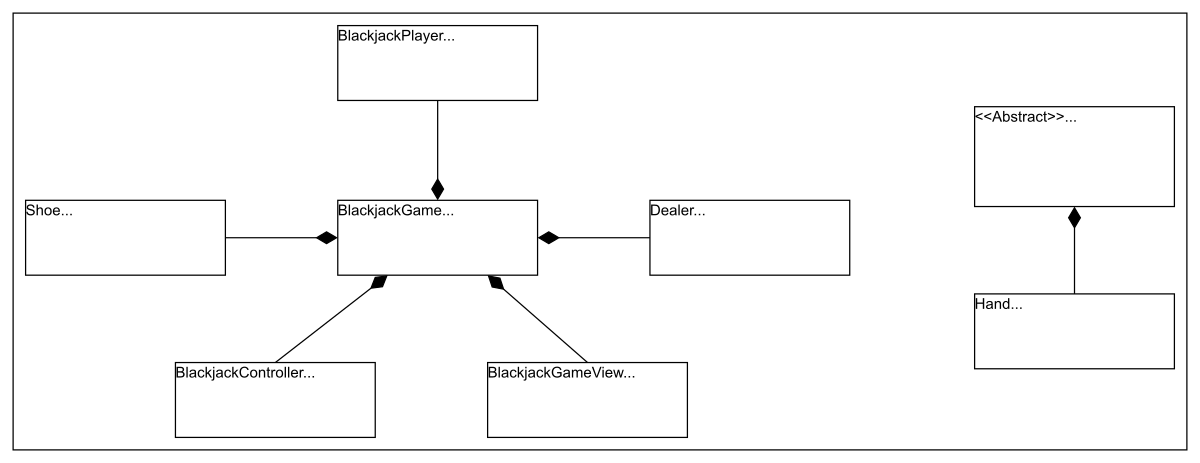
\includegraphics[width=0.5\textwidth]{Images/chapter_12/section_4902989846544384/4917396698431488.png}
 \caption{The composition relationship between classes}
\end{figure}

\subsubsection{Inheritance}\label{VB-a0gzbl1Vlz8sozqCrS}
\\
The following classes show an inheritance relationship:

\begin{itemize}
\item
\protect\phantomsection\label{Y6ibHxjk26nffF_0Z6qLn}
\texttt{BlackjackPlayer} and \texttt{Dealer} both \emph{inherit} from \texttt{Player}.

\begin{itemize}
\item
This means both subclasses share fields such as \texttt{id}, \texttt{password}, \texttt{balance}, \texttt{status}, \texttt{person}, and \texttt{hand}, and may implement or override behaviors like \texttt{resetPassword()}.
\end{itemize}
\end{itemize}
\begin{quote}
\textbf{Note:} We have already discussed the inheritance relationship between classes in the component section above one by one.
\end{quote}
\subsection{Class diagram for the Blackjack game}\label{bstILSbPAlow9Symxkzr6}
\\
This section outlines the multiplicity (cardinality) relationships between the main classes in our Blackjack game. We explain the allowed number of instances on each side for each relationship and the real-world or design rationale behind the connection. Understanding these relationships is key to modeling how different entities interact and collaborate to support key workflows in the system.

\begin{center}
\begin{tabular}{|p{0.22\linewidth}|p{0.22\linewidth}|p{0.18\linewidth}|p{0.30\linewidth}|}
\hline
\textbf{Source} & \textbf{Target} & \textbf{Multiplicity} & \textbf{Reason} \\
\hline

Shoe & Deck & 1--1..* & A Shoe contains one or more decks (usually 4–8 in casinos). \\
\hline

Deck & Card & 1--52 & Each Deck always contains exactly 52 cards. \\
\hline

Hand & Card & 1--2..* & A Hand has at least 2 cards, but may have more due to hits or splits. \\
\hline

Player (abstract) & Hand & 1--1 & Each Player has exactly one Hand (may be 1--1..* if splits are supported). \\
\hline

BlackjackGame & Shoe & 1--1 & Each game session uses exactly one Shoe. \\
\hline

BlackjackGame & BlackjackPlayer & 1--1..* & A game has one or more BlackjackPlayers. \\
\hline

BlackjackGame & Dealer & 1--1 & Each game has exactly one Dealer. \\
\hline

BlackjackGame & BlackjackController & 1--1 & Each session has one Controller handling actions. \\
\hline

BlackjackGame & BlackjackGameView & 1--1 & Each game has exactly one GameView for displaying state. \\
\hline

\end{tabular}
\end{center}


Here's the complete class diagram for our Blackjack game:

\begin{figure}[htbp]
 \centering
 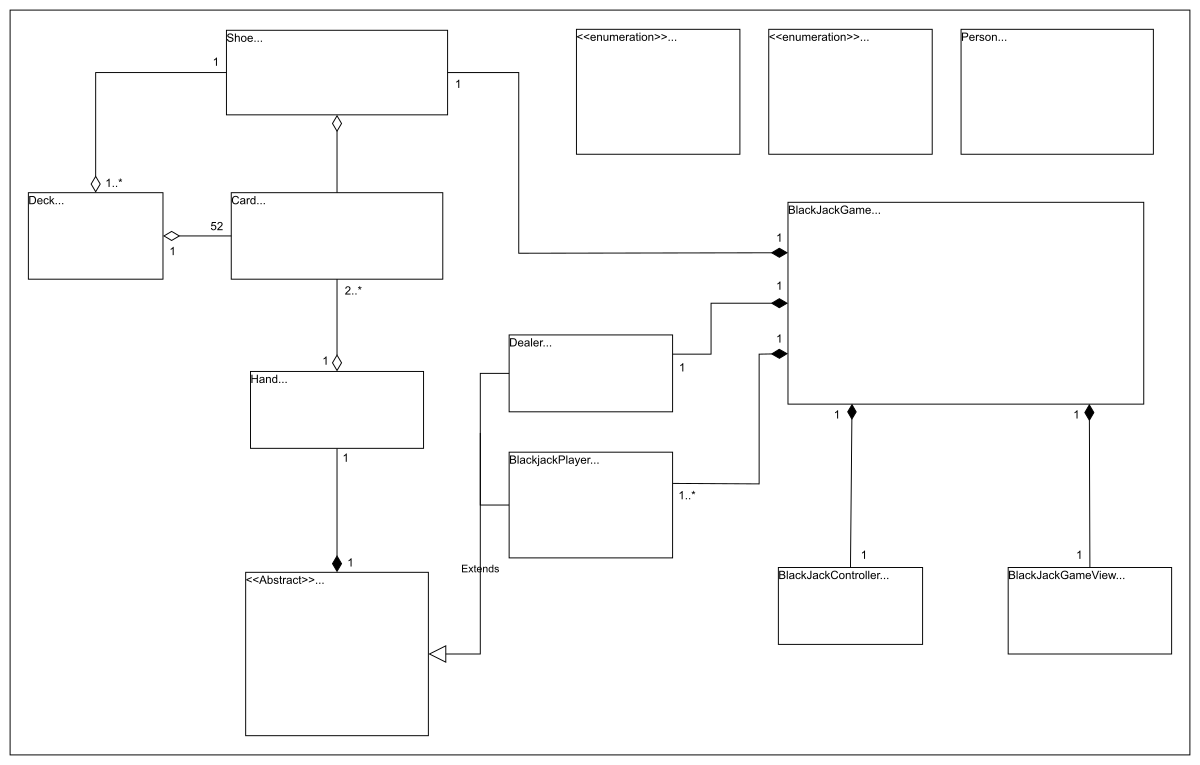
\includegraphics[width=0.5\textwidth]{Images/chapter_12/section_4902989846544384/6590625930412032.png}
 \caption{The class diagram of the Blackjack game}
\end{figure}

\subsection{Design pattern}\label{1JdnBslPYoJ3idant5lQ4}
\\
The Iterator design pattern is highly relevant to our Blackjack game. It allows sequential access to the elements in a collection---such as a deck or shoe---without exposing the underlying data structure.
\begin{quote}
\textbf{For example:} When dealing cards from the deck or shoe, the system simply iterates through the collection of cards, handing them out to each player and the dealer. This cleanly separates the card distribution logic from the internal representation of the deck or shoe, promoting encapsulation and flexibility.
\end{quote}
\\
The State design pattern is also applicable and beneficial for managing the game's progression. Blackjack is a classic example of a system that transitions through a series of well-defined states. By encapsulating each state as a distinct object, the State pattern allows the game to alter its behavior when its internal state changes, without relying on complex conditionals.
\\
Some of the core states in an online Blackjack game might include:

\begin{itemize}
\item
\protect\phantomsection\label{r5vkLw9gDbeZlDZtzVZtb}
\textbf{Shuffling:} The system shuffles the shoe (or decks) before starting a round.
\item
\protect\phantomsection\label{KcYa7_1hR0WHYtX-zEJBv}
\textbf{Dealing:} Cards are distributed to the dealer and all players.
\item
\protect\phantomsection\label{ncNtm5HSfXUS-UWB6dcgb}
\textbf{Player's Turn:} The player can choose to hit (draw a card) or stand.
\item
\protect\phantomsection\label{EQszoWNGJlw7U4tV4DPHF}
\textbf{Dealer's Turn:} The dealer reveals cards and follows house rules (e.g., must hit until reaching 17).
\item
\protect\phantomsection\label{PPT2lUtfyX7F8VZYP4tsC}
\textbf{Settlement:} The game evaluates outcomes (win, lose, push), pays out winnings, and collects losses.
\item
\protect\phantomsection\label{fMQmo3Vux3gFv2Op62MHb}
\textbf{Game Over:} The round ends, and the system prepares for a new game or round.
\end{itemize}
\\
Implementing the state pattern allows each stage to be managed as a separate state object, making the game engine more modular, maintainable, and easy to extend for additional rules or variants.

\subsection{AI-powered trainer}\label{dIPd6IMbJsoDHgzfmZe8_}
\\
At this stage, everything should be clear. If you encounter any confusion or ambiguity, feel free to utilize the interactive AI-enabled widget below to seek clarification. This tool is designed to help you strengthen your understanding of the concepts.

\begin{figure}[htbp]
 \centering
 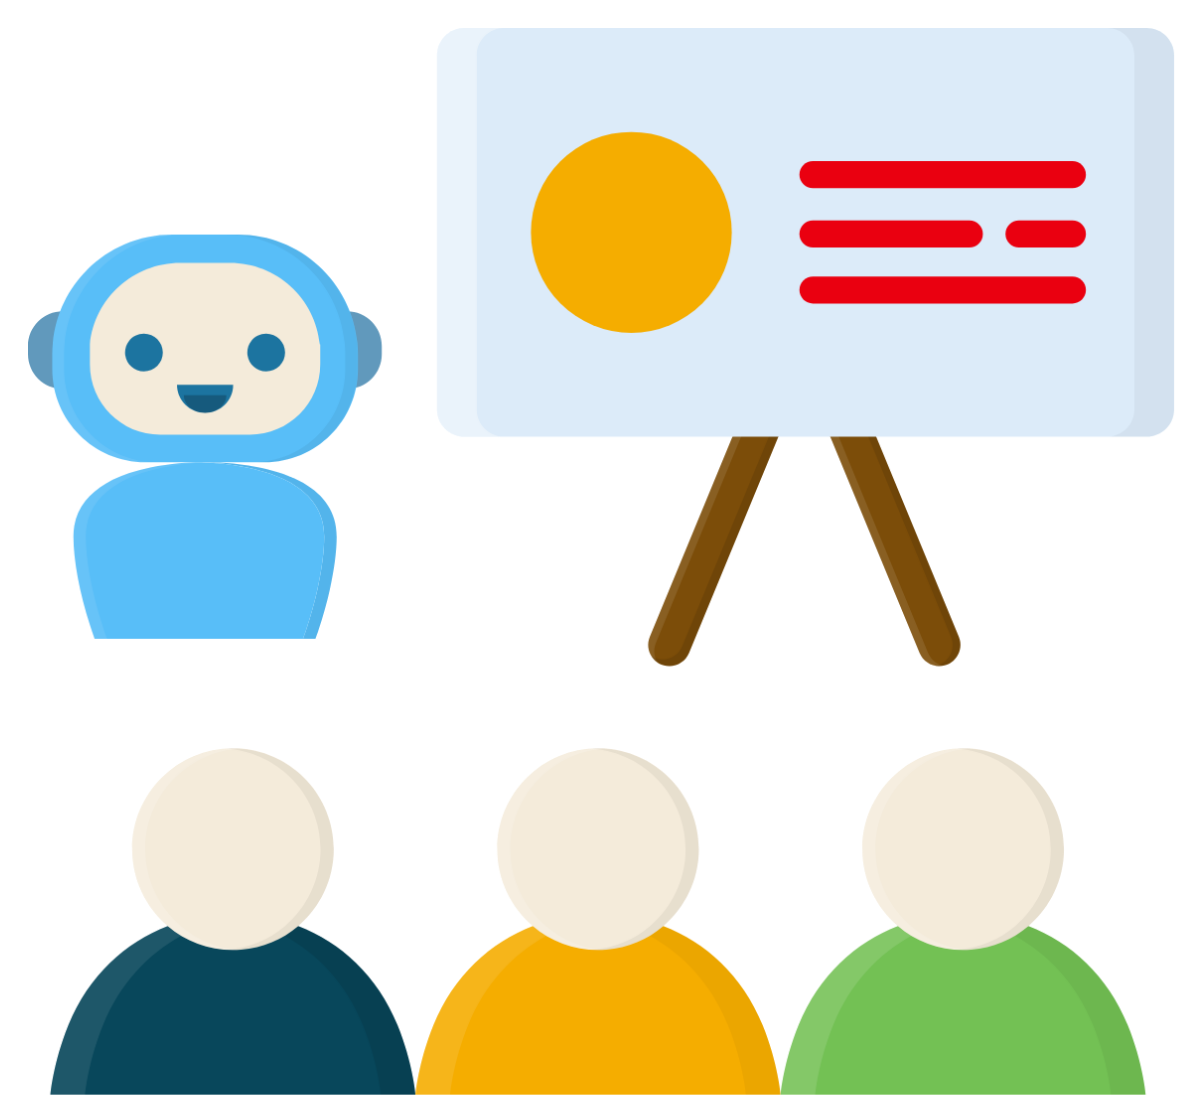
\includegraphics[width=0.15\textwidth]{Images/chapter_12/section_4902989846544384/5773798916620288.png}
 
\end{figure}

We have completed the class diagram of the Blackjack game according to the requirements. In the next lesson, let's design the activity diagram of the Blackjack game.

% End of section content